% Figure "reduction" of "Galashin's Conjecture 4.3 via a convex gradient": (a) the crossing graph of the window
% (3,1,2,6,4,5) has two components, each with its least label; (b) deleting a loop (CLH-1, component reduction and loops).
% Source in the paper's own fonts at the text width (6.5in = 468bp). It adds no assertion.
% Every value drawn is read from Lean output lines (SHA-256 of the lines):
%   picture D106 50526015e20e6f184a3f35493e09c7333d79d3dee392c9a629350e93d398a355   (Conj43.crossEdges of the window (3,1,2,6,4,5))
%   picture D103 cb53562d56ac3706682bb6d5d23a7d9db5134c218833d2e235d83ba248fc75e8   (n=5, loop 3: length and rank of the affine lift)
% Panel (a) is evaluated by the formal definitions; the length and rank in panel (b) are integer counts made in Lean.
% Build: pdflatex <this file> && pdftocairo -svg <this file>.pdf <this file>.svg
\documentclass[11pt]{standalone}
\usepackage[T1]{fontenc}
\usepackage{lmodern}
\usepackage{amsmath,amssymb}
\usepackage{tikz}
\usetikzlibrary{arrows.meta,positioning,calc}

% the palette of the paper's other figures: blue solid for the first strand, cycle or arc, ochre dashed for the second
\definecolor{ink}{HTML}{233740}
\definecolor{muted}{HTML}{65757D}
\definecolor{pblue}{HTML}{0072B2}
\definecolor{qochre}{HTML}{B87827}

\tikzset{
  base/.style={draw=muted, line width=0.5pt},
  ttl/.style={font=\small, text=ink, inner sep=0pt},
  lab/.style={font=\footnotesize, inner sep=1.2pt, text=ink},
  labm/.style={font=\small, inner sep=1.2pt, text=ink},
  labP/.style={font=\small, inner sep=1.2pt, text=pblue},
  labQ/.style={font=\small, inner sep=1.2pt, text=qochre},
  idx/.style={font=\footnotesize, text=muted, inner sep=0pt},
  negE/.style={font=\small, text=pblue, inner sep=0pt},
  posE/.style={font=\small, text=qochre, inner sep=0pt},
  zeroE/.style={font=\small, text=muted, inner sep=0pt},
  vtx/.style={circle, draw=ink, fill=white, line width=0.6pt, inner sep=0pt, minimum size=16bp, font=\small, text=ink},
  cycP/.style={pblue, line width=1.1pt, -{Stealth[length=5pt,width=4.2pt]}, shorten >=1pt, shorten <=1pt},
  cycQ/.style={qochre, line width=1.1pt, dash pattern=on 4pt off 1.6pt, -{Stealth[length=5pt,width=4.2pt]}, shorten >=1pt, shorten <=1pt},
  chord/.style={pblue, line width=0.9pt},
  arrP/.style={pblue, line width=1.0pt, -{Stealth[length=4.4pt,width=3.8pt]}},
  arrQ/.style={qochre, line width=1.0pt, dash pattern=on 4pt off 1.6pt, -{Stealth[length=4.4pt,width=3.8pt]}},
  arrM/.style={muted, line width=0.6pt, -{Stealth[length=4pt,width=3.4pt]}},
}

\begin{document}
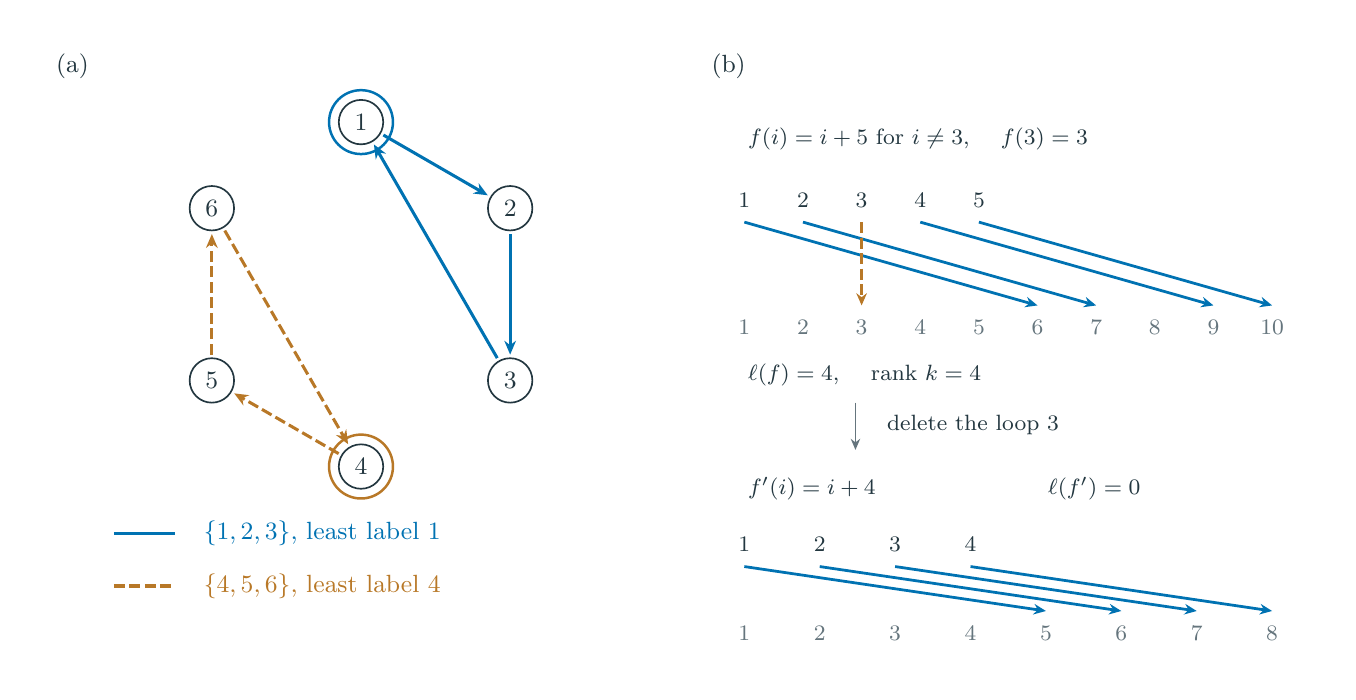
\begin{tikzpicture}[x=1bp,y=1bp]
\useasboundingbox (0,0) rectangle (468.000,232.000); %@ red canvas w=468.000 h=232.000
\node[ttl,anchor=west] at (10.000,218.000) {(a)};
\node[ttl,anchor=west] at (246.000,218.000) {(b)};
\node[vtx] (a1) at (120.000,198.000) {1}; %@ red vtx label=1 x=120.000 y=34.000
\node[vtx] (a2) at (173.694,167.000) {2}; %@ red vtx label=2 x=173.694 y=65.000
\node[vtx] (a3) at (173.694,105.000) {3}; %@ red vtx label=3 x=173.694 y=127.000
\node[vtx] (a4) at (120.000,74.000) {4}; %@ red vtx label=4 x=120.000 y=158.000
\node[vtx] (a5) at (66.306,105.000) {5}; %@ red vtx label=5 x=66.306 y=127.000
\node[vtx] (a6) at (66.306,167.000) {6}; %@ red vtx label=6 x=66.306 y=65.000
\draw[cycP] (a1) -- (a2); %@ red edge p=1 q=2 comp=0
\draw[cycP] (a2) -- (a3); %@ red edge p=2 q=3 comp=0
\draw[cycP] (a3) -- (a1); %@ red edge p=3 q=1 comp=0
\draw[cycQ] (a4) -- (a5); %@ red edge p=4 q=5 comp=1
\draw[cycQ] (a5) -- (a6); %@ red edge p=5 q=6 comp=1
\draw[cycQ] (a6) -- (a4); %@ red edge p=6 q=4 comp=1
\draw[pblue, line width=0.9pt] (a1) circle (11.5bp); %@ red anchor label=1 comp=0
\draw[qochre, line width=0.9pt] (a4) circle (11.5bp); %@ red anchor label=4 comp=1
\draw[cycP, -] (30.000,50.000) -- (54.000,50.000);
\node[labP,anchor=west] at (62.000,50.000) {$\{1,2,3\}$, least label 1}; %@ red legend comp=0 members=1,2,3 anchor=1
\draw[cycQ, -] (30.000,31.000) -- (54.000,31.000);
\node[labQ,anchor=west] at (62.000,31.000) {$\{4,5,6\}$, least label 4}; %@ red legend comp=1 members=4,5,6 anchor=4
\node[lab,anchor=west] at (258.000,192.000) {$f(i)=i+5$ for $i\ne3$, \quad $f(3)=3$}; %@ red before f=i+5 loop=3
\node[lab] at (258.000,170.000) {$1$}; %@ red before top k=1 x=258.000
\node[lab] at (279.111,170.000) {$2$}; %@ red before top k=2 x=279.111
\node[lab] at (300.222,170.000) {$3$}; %@ red before top k=3 x=300.222
\node[lab] at (321.333,170.000) {$4$}; %@ red before top k=4 x=321.333
\node[lab] at (342.444,170.000) {$5$}; %@ red before top k=5 x=342.444
\node[idx,font=\footnotesize] at (258.000,124.000) {$1$}; %@ red before bot k=1 x=258.000
\node[idx,font=\footnotesize] at (279.111,124.000) {$2$}; %@ red before bot k=2 x=279.111
\node[idx,font=\footnotesize] at (300.222,124.000) {$3$}; %@ red before bot k=3 x=300.222
\node[idx,font=\footnotesize] at (321.333,124.000) {$4$}; %@ red before bot k=4 x=321.333
\node[idx,font=\footnotesize] at (342.444,124.000) {$5$}; %@ red before bot k=5 x=342.444
\node[idx,font=\footnotesize] at (363.556,124.000) {$6$}; %@ red before bot k=6 x=363.556
\node[idx,font=\footnotesize] at (384.667,124.000) {$7$}; %@ red before bot k=7 x=384.667
\node[idx,font=\footnotesize] at (405.778,124.000) {$8$}; %@ red before bot k=8 x=405.778
\node[idx,font=\footnotesize] at (426.889,124.000) {$9$}; %@ red before bot k=9 x=426.889
\node[idx,font=\footnotesize] at (448.000,124.000) {$10$}; %@ red before bot k=10 x=448.000
\draw[arrP] (258.000,162.000) -- (363.556,132.000); %@ red before arrow from=1 to=6 dest=363.556
\draw[arrP] (279.111,162.000) -- (384.667,132.000); %@ red before arrow from=2 to=7 dest=384.667
\draw[arrQ] (300.222,162.000) -- (300.222,132.000); %@ red before arrow from=3 to=3 dest=300.222
\draw[arrP] (321.333,162.000) -- (426.889,132.000); %@ red before arrow from=4 to=9 dest=426.889
\draw[arrP] (342.444,162.000) -- (448.000,132.000); %@ red before arrow from=5 to=10 dest=448.000
\node[lab,anchor=west] at (258.000,107.000) {$\ell(f)=4$, \quad rank $k=4$}; %@ red before length=4 rank=4
\draw[arrM] (298.000,97.000) -- (298.000,80.000);
\node[lab,anchor=west] at (308.000,89.000) {delete the loop $3$};
\node[lab,anchor=west] at (258.000,66.000) {$f'(i)=i+4$}; %@ red after f=i+4
\node[lab] at (258.000,46.000) {$1$}; %@ red after top k=1 x=258.000
\node[lab] at (285.143,46.000) {$2$}; %@ red after top k=2 x=285.143
\node[lab] at (312.286,46.000) {$3$}; %@ red after top k=3 x=312.286
\node[lab] at (339.429,46.000) {$4$}; %@ red after top k=4 x=339.429
\node[idx,font=\footnotesize] at (258.000,14.000) {$1$}; %@ red after bot k=1 x=258.000
\node[idx,font=\footnotesize] at (285.143,14.000) {$2$}; %@ red after bot k=2 x=285.143
\node[idx,font=\footnotesize] at (312.286,14.000) {$3$}; %@ red after bot k=3 x=312.286
\node[idx,font=\footnotesize] at (339.429,14.000) {$4$}; %@ red after bot k=4 x=339.429
\node[idx,font=\footnotesize] at (366.571,14.000) {$5$}; %@ red after bot k=5 x=366.571
\node[idx,font=\footnotesize] at (393.714,14.000) {$6$}; %@ red after bot k=6 x=393.714
\node[idx,font=\footnotesize] at (420.857,14.000) {$7$}; %@ red after bot k=7 x=420.857
\node[idx,font=\footnotesize] at (448.000,14.000) {$8$}; %@ red after bot k=8 x=448.000
\draw[arrP] (258.000,38.000) -- (366.571,22.000); %@ red after arrow from=1 to=5 dest=366.571
\draw[arrP] (285.143,38.000) -- (393.714,22.000); %@ red after arrow from=2 to=6 dest=393.714
\draw[arrP] (312.286,38.000) -- (420.857,22.000); %@ red after arrow from=3 to=7 dest=420.857
\draw[arrP] (339.429,38.000) -- (448.000,22.000); %@ red after arrow from=4 to=8 dest=448.000
\node[lab,anchor=west] at (366.000,66.000) {$\ell(f')=0$}; %@ red after length=0
\end{tikzpicture}
\end{document}
